% Chapter Template

\chapter{Introduction} % Main chapter title

\label{Chapter1} % Change X to a consecutive number; for referencing this chapter elsewhere, use \ref{ChapterX}

\lhead{Chapter 1. \emph{Introduction}} % Change X to a consecutive number; this is for the header on each page - perhaps a shortened title

%----------------------------------------------------------------------------------------
%	SECTION 1 - Voice Activity Detection
%----------------------------------------------------------------------------------------

\section{Voice Activity Detection}

Voice Activity Detection (VAD) is a process of identifying parts of an audio recording which contain the presence of human voice as opposed to those which are only comprised of silence or the background noise. VAD is a relatively simple task in recordings which have high signal-to-noise ratios (SNR), in which voice can be distinguished from noise simply by computing the short-time energy of all frames and setting an appropriate threshold for their classification. However, in real applications, the signal is almost always corrupted to some extent by background noise which makes the VAD performance to deteriorate. VAD decision is especially difficult for the unvoiced phonemes \cite{Kondoz} whose spectrum contains no periodicity and is often similar to the one of white noise \cite{Michaelis}.

There has been an active research in the VAD area from as early as 1975, when Rabiner and Sambur \cite{RabinerSambur} proposed a VAD algorithm (then referred to as "algorithm for determining the endpoints of isolated utterances") based on the aforementioned short-time energy and the zero-crossing rate. This approach worked reasonably well for signals with SNR on the order of 30 dB, however since then there has been a need for much better performance, including applications where algorithm robustness has to be achieved even at negative SNRs. Recently, numerous VAD approaches have been proposed, based on various features such as ..... ..... ..... . 

%----------------------------------------------------------------------------------------
%	SECTION 2 - Applications of VAD
%----------------------------------------------------------------------------------------

\section{Applications of VAD}

VAD is often the first step in many signal processing applications including speech recognition \cite{RamirezGorriz, Kuroiwa, Martin, Shafran, RamirezGorrizArt}, speech coding and transmission \cite{Sohn, RamirezGorriz, Prasad, G729, GSMControl}, speech enhancement \cite{Park, RamirezGorriz, Borisagar}, noise estimation \cite{RamirezGorriz} or speaker recognition \cite{Sahidullah}. In most applications the noise-robust VAD decisions reduce the computational load required by the system and improve its accuracy. The reduced computational load is achieved since the voice-inactive frames are often not processed at all. At the same time, the clear boundaries of an utterance help to improve the accuracy of some systems (e.g. speech recognition).

\subsection{Automatic Speech Recognition}

In Automatic Speech Recognition (ASR), it is of importance to first extract the voice-active parts of a signal which can then be passed to the actual recognition module. This procedure increases both the accuracy of the ASR system as well as its speed, since the recognition task is not performed on the parts of the signal which do not contain speech. A sample block diagram of an ASR system which uses a VAD module is presented in Figure \ref{fig:ASRVAD} \cite{RamirezGorriz}. For ASR, and also most other applications, it is crucial for the VAD module to be able to identify all speech segments in order not to degrade the accuracy of the entire ASR system. Therefore, VAD systems often implement a fail-safe approach which means that if there is an uncertainty in classification of a frame, it is safer to label is as speech than otherwise. Typically, there is a trade-off in VAD performance which can be characterised as maximising the precision while keeping the recall at a steady, high rate.

\begin{figure}[htbp]
	\centering
		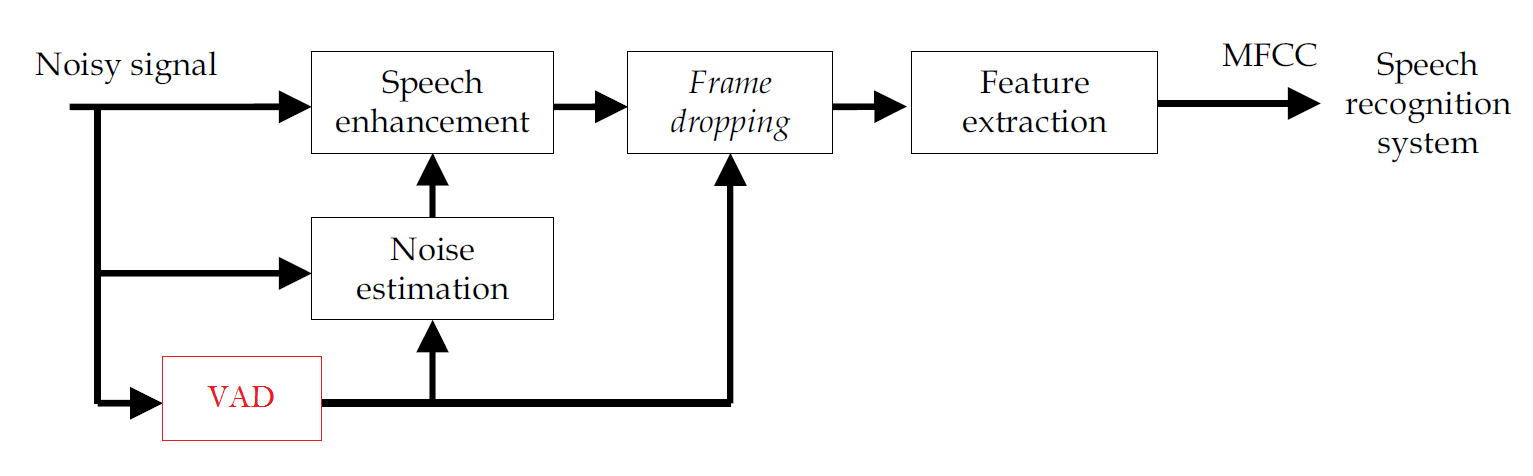
\includegraphics[width=1\columnwidth]{Figures/ASRVAD.png}
		\rule{37em}{0.5pt}
	\caption[Automatic Speech Recognition system with Voice Activity Detection module]{Block diagram of an Automatic Speech Recognition system with Voice Activity Detection module \cite{RamirezGorriz}}
	\label{fig:ASRVAD}
\end{figure}

\subsection{Speech Coding and Transmission}

It has been calculated that during a typical phone conversation each person speaks, on average, no more than 50\% of the time \citep{GSMControl}. Therefore, signal transmission would be greatly optimised if each transmitter could be switched-off half of the time, causing the system capacity to double. Such approach is known as discontinuous transmission (DTX). Alternatively, a dual-mode encoding technique could be employed, which uses a higher bit-rate for coding the voice-active frames and lower for silence/noise.

Figure \ref{fig:DTXVAD} shows a structure of a dual-mode coding and transmission system, in which the VAD module is used to direct the incoming signal into either the active or inactive speech encoder. The noise can be either transmitted at a much lower bit-rate or the transmission might be switched off completely. In case of a stopped transmission, the receiving end often implements a \emph{comfort noise} \citep{GSMControl,RamirezGorriz} generation module, which creates a synthetic signal similar to the background noise at the transmitter so that the listener does not notice the rapid, inconvenient switching during the conversation.

\begin{figure}[htbp]
	\centering
		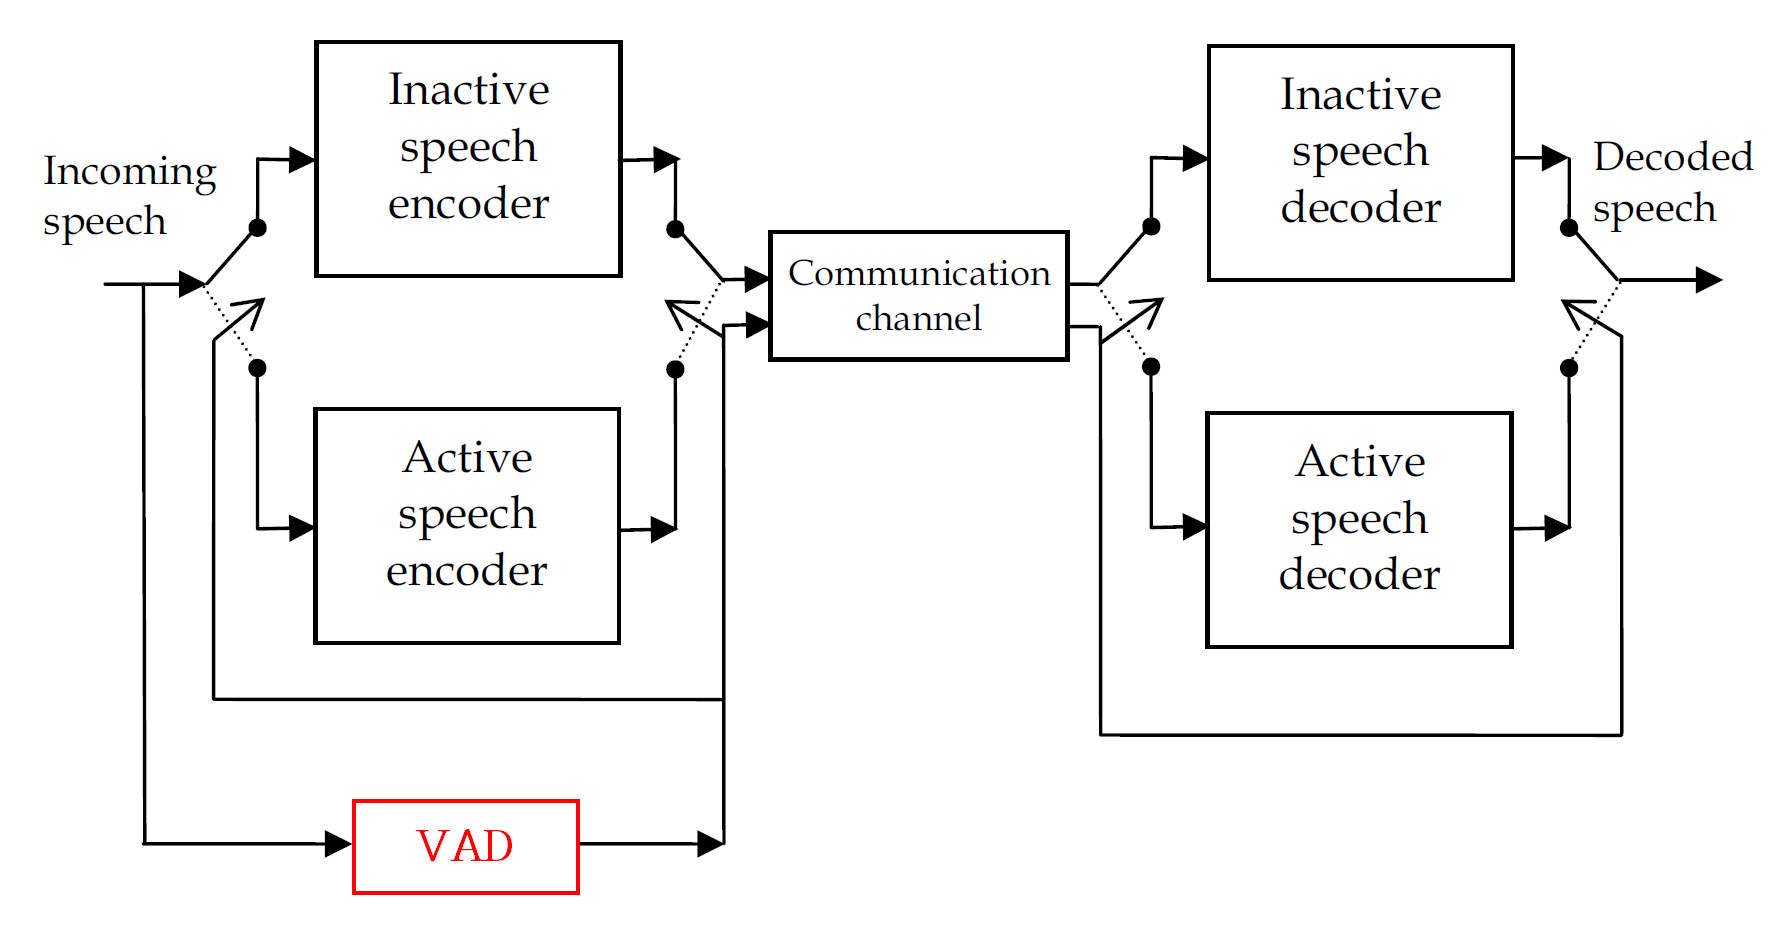
\includegraphics[width=1\columnwidth]{Figures/DTXVAD.png}
		\rule{37em}{0.5pt}
	\caption[Dual-mode transmission system with Voice Activity Detection module]{Block diagram of an dual-mode transmission system with Voice Activity Detection module \cite{RamirezGorriz}}
	\label{fig:DTXVAD}
\end{figure}

\subsection{Noise Estimation and Speech Enhancement}

Speech enhancement aims to improve the intelligibility and quality of speech signals corrupted by additive  noise of some kind. Many speech enhancement systems use a technique called \emph{spectral subtraction} \cite{Kondoz, RamirezGorriz}. It assumes, that the clean speech can be represented in the frequency-domain in the form:
\begin{equation}
|S(f)| = |Y(f)| - |N(f)|
\end{equation}
where $|Y(f)|$ is the amplitude spectrum of the corrupted speech, $|S(f)|$ of the clean speech and $|N(f)|$ of the noise. In order for this technique to work, the noise needs to be additive, stationary and uncorrelated with the clean speech signal. Additionally, one needs to know the spectrum of the noise, which in real-world applications where a variety of different noise types are encountered, is a nontrivial problem. A robust Voice Activity Detector can become very useful in this task by identifying the voice-inactive frames of a signal from which the noise statistics could be estimated.

%----------------------------------------------------------------------------------------
%	SECTION 3 - Structure of a typical VAD system
%----------------------------------------------------------------------------------------

\section{Structure of a typical VAD system}

Figure \ref{fig:VADStructure} shows a high-level structure of a Voice Activity Detector, however only the two middle blocks are considered a core of a typical VAD system. The noisy speech signal is passed to a pre-processing module which might perform a variety of processing tasks, including noise estimation and suppression in order to improve the performance of the actual VAD algorithm. Additionally, during pre-processing the signal is often split into frames which are typically 20-100 ms long. In the next step, 

\begin{figure}[htbp]
	\centering
		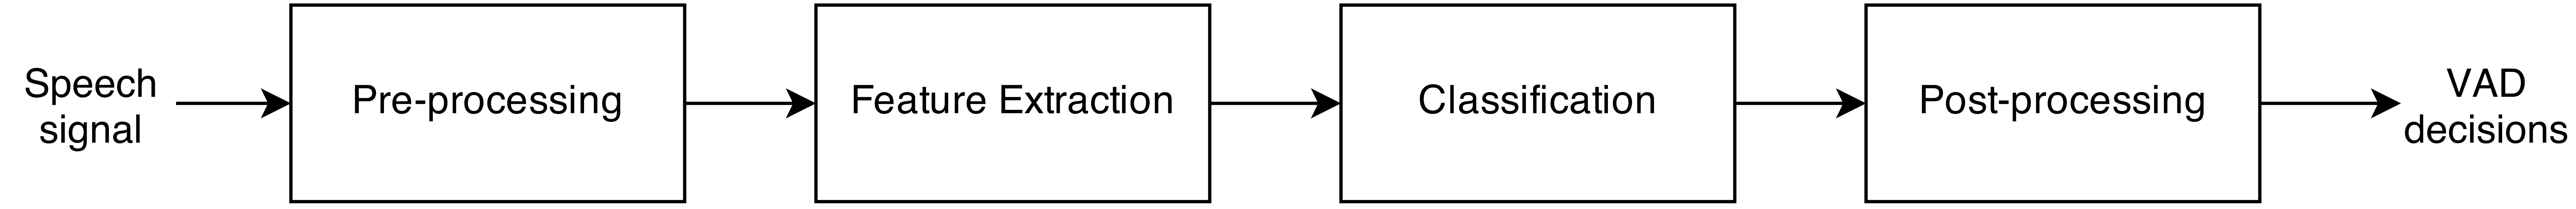
\includegraphics[width=1\columnwidth]{Figures/VADStructure.png}
		\rule{37em}{0.5pt}
	\caption[Block diagram of a typical Voice Activity Detection system]{Block diagram of a typical Voice Activity Detection system}
	\label{fig:VADStructure}
\end{figure}